\documentclass[a4paper,10pt]{book}
\usepackage[utf8x]{inputenc}
% User defined settings
\usepackage{xspace}
\usepackage{psfrag}
\usepackage{xcolor}
\usepackage{natbib}
\usepackage{tabularx}
\usepackage{multicol}
\usepackage[verbose]{wrapfig}
\usepackage[colorlinks,bookmarks=true]{hyperref}
\usepackage{amsbsy,amsfonts,amsmath,amssymb,enumerate,epsfig,graphicx,rotating}
\usepackage[FIGTOPCAP,nooneline]{subfigure}
% \usepackage{mdframed}

%Mathematics
\newcommand{\f}[2]{\frac{#1}{#2}}
\newcommand{\dd}{\partial}
\newcommand{\de}{{\rm \, d}}
\newcommand{\mysec}[1]{{\noindent\bf #1.}}
\newcommand{\pn}{Prandtl number}
%-------- Vectors
\renewcommand{\vec}[1]{\mathbf{#1}}
\renewcommand{\v}{\vec}
\newcommand{\bec}{\vec}

%-------- Numbers
\newcommand{\Ra}{$Ra\ $}
\renewcommand{\P}{$P\ $}
\newcommand{\Nu}{$Nu\ $}
\renewcommand{\t}{$\tau\ $}
\newcommand{\Pm}{$P_m\ $}
\newcommand{\El}{$\Lambda\ $}
\newcommand\ie{i.e.\ }
\newcommand\etal{\mbox{\textit{et al.}}}
\newcommand\etc{etc.\ }
\newcommand\eg{e.g.\ }
\newcommand{\mypsfrag}[2]{\psfrag{#1}{\footnotesize{#2}}}
\newcommand{\warningbox}[1]{\fcolorbox{orange}{white}%
{\centering \parbox{0.9\textwidth}{ {\Large \red{Warning}}%
\vspace*{2mm}\\%
#1}}}


\providecommand{\MD}{\textbf{MD}\xspace}
\providecommand{\FD}{\textbf{FD}\xspace}
\providecommand{\Mdip}{\ensuremath{{M}_\text{dip}}\xspace}
\providecommand{\Mmp}{\ensuremath{\overline{M}_p}\xspace}
\providecommand{\Mft}{\ensuremath{\widetilde{M}_t}\xspace}
\providecommand{\Mmt}{\ensuremath{\overline{M}_t}\xspace}
\providecommand{\Mfp}{\ensuremath{\widetilde{M}_p}\xspace}
\providecommand{\Emp}{\ensuremath{\overline{E}_p}\xspace}
\providecommand{\Efp}{\ensuremath{\widetilde{E}_p}\xspace}
\providecommand{\Emt}{\ensuremath{\overline{E}_t}\xspace}
\providecommand{\Eft}{\ensuremath{\widetilde{E}_t}\xspace}
\providecommand{\Ha}{\ensuremath{H_{\vec{_a}}}\xspace}
\providecommand{\Hu}{\ensuremath{H_{\vec{_u}}}\xspace}
\providecommand{\HB}{\ensuremath{H_{\vec{_B}}}\xspace}
\providecommand{\Hcross}{\ensuremath{H_\times}\xspace}
\providecommand{\MfpToMmp}{\ensuremath{\widetilde{M}_p/\overline{M}_p}\xspace}
\providecommand{\MfpToMmpD}{\ensuremath{\widetilde{M}_p^\mathrm{dip}/\overline{M
}_p^\mathrm{dip}}\xspace}


\newcommand\red[1]{{\color{red} #1}}
\newcommand\todo[2]{{\color{red} #1 \\ {\rule{1mm}{0mm} \hfill ACTION: #2}}}

\allowdisplaybreaks
\usepackage{charter}

\title{GLO ($@GLO_VERSION@$) \\ A User's Manual}
\author{Luis Silva}

\begin{document}

\pagenumbering{alph}

\maketitle

\clearpage\pagenumbering{roman}

\tableofcontents

\clearpage\pagenumbering{arabic}
\chapter*{Introduction}
\addcontentsline{toc}{chapter}{Introduction}
This is the user manual for the GLO (\underline{G}lasgow \underline{L}inear \underline{O}set) code.
API documentation can be found on the online APIDOX.
Ported to f95 by Luis Silva (lacsilva@gmail.com)

\chapter{How to use this code}

\section{DEPENDENCIES}
We use cmake version 2.6-patch 4 as the build system.
For optimisation purposes, we ship our own copy of the required lapack
subroutines and their dependencies. Speciffically, we depend on the subroutine
\verb|zggev| \url{http://www.netlib.org/lapack/explore-3.1.1-html/zggev.f.html}
Online documentation can be built using doxygen $>=$ 1.6.1

\section{Compiling and installing the code}
The GLO code and utilities use the cmake build system in order to generate
native builds for *nix and Windows alike. Some features can be activated or
deactivated at compile time by passing the appropriate ``-D'' option to cmake.
Check the cmake documentation \citep{CMakeDox} for other build options.

\subsection{Building the online documentation}
\begin{verbatim}
$ mkdir BUILD
$ cd BUILD
$ cmake ..
$ make doc
\end{verbatim}
The code documentation can then be found by pointing a browser
to:\\
\verb|<your favorite browser> BUILD/APIDOX/index.html|

\subsection{COMPILATION}
\begin{verbatim}
$ mkdir BUILD
$ cd BUILD
$ cmake ..
$ make && make install
\end{verbatim}
After all run successfully, the file drs.exe should be in \verb|bin/|.

\section{Running GLO}
\subsection{Before running GLO}
\label{s:runConfig}
Each run needs to be configured. Configuration is passed on the standard input
and obeys a format similar to the following.
\begin{tiny}
\begin{verbatim}
Symmetry = 2
Calculation = 3
VariablePar = Rt
Rt = 3.0e6 
tau = 1.0e5 
Pt = 1.0 
eta = 0.35 
Le = 0.3 
Rc = 1.0e2
Truncation = 10 
m0 = 19
AbsParameterError = 1.00E-08 
RelativeGRError = 1.00E-03 
MaxIterations = 1000
StepSize = -100 
UpperLimit = 9.97e4
\end{verbatim}
\end{tiny}

Calculation can assume integer values between -1 and 7 as described below:

\begin{tabular}{| m{0.1\textwidth} | p{0.8\textwidth}|}
Value & Descrition \\ \hline
-1  &  {Varies the specified parameter and computes the growth rate for 
other parameters fixed. The step size is taken to be the order of magnitude 
of the value of the parameter (for example, if we are steping in Rt and Rt 
is $5\times10^3$, then the step size is $10^3$). The step size is never 
smaller than \verb|StepSize|.}\\
\end{tabular}

\chapter{Theory}

\section{Problem set up and approximations}
\label{s:problemSetup}
We consider a spherical fluid shell of inner radius $r_i$ and outer radius
$r_o$. The shell thickness is then $d = r_o - r_i$. The shell is rotating at
constant angular velocity $\Omega$ about an axis aligned with the $z$ direction.
Boundaries are impermeable and electrically insulating. Figure~\ref{f:setup}
\begin{figure}[htb]
\centering
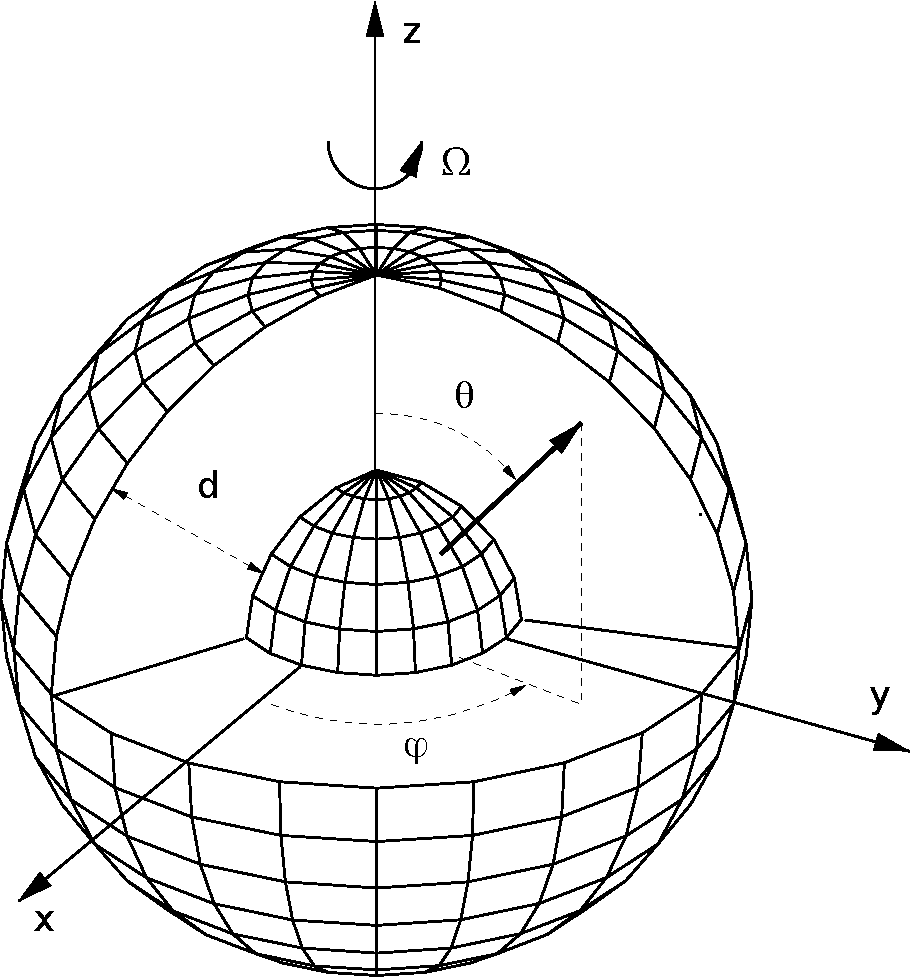
\includegraphics[width=0.5\textwidth]{figs/sphshell}
\caption{Depiction of the problem set-up.}
\label{f:setup}
\end{figure}

The fluid inside the shell is electrically and thermally conductive with
magnetic diffusivity $\lambda$ and thermal diffusivity $\kappa$, and has a
viscosity $\nu$. It is assumed to have a static thermal state described by a
radial temperature profile $T_S (r)$ that can be one of the values described in
Table~\ref{t:t_profiles}.
\begin{table}[htb]
\centering
\begin{tabular}{|c|lp{0.48\textwidth}|}\hline
 Opt. & Equation & Description\\\hline
  &                          & \\
 0&$T_S(r) = T_0 + \beta(r_i r_o/r - r_i)$ & The conductive temperature
 profile used in \citep{ChristensenEtAl01}.
 \\\hline
  &                          & \\
 1&$T_S(r) = T_0 - \beta r^2/2$    & This profile closely
follows the adiabat \citep{LabrossePoirier1997,DaviesGubbins2011} and alludes to
the possibility that at least a fraction of the energy available to planetary
dynamos is due to radiogenic heat release. \\ \hline
\end{tabular}
\caption{Possible temperature profiles, in K, hardcoded into GLO. First column
refers to the option values used in the code.}
\label{t:t_profiles}
\end{table}

Constants $T_0$ and $\beta$ have values that depend on the profile and can be
written, in dimensional form, as a function of the temperature at the top
($T_o$) and bottom ($T_i$) boundaries. Opt.~0 has $T_0 = T_o$ and $\beta = (T_i
-T_o)/d$ and refers to the same temperature profile used in the first dynamo
benchmark exercise \citep{ChristensenEtAl01} whereas Opt.~1 has $T_0 = (T_i
r_o^2 - T_o r_i^2)/(r_o^2 - r_i^2)$ and $\beta = (T_o - T_i)/(r_o^2 - r_i^2)$,
thus closely following an adiabatic temperature profile
\citep{LabrossePoirier1997, DaviesGubbins2011}.

\begin{figure}[htb]
\centering
 % GNUPLOT: LaTeX picture
\setlength{\unitlength}{0.240900pt}
\ifx\plotpoint\undefined\newsavebox{\plotpoint}\fi
\begin{picture}(1500,900)(0,0)
\sbox{\plotpoint}{\rule[-0.200pt]{0.400pt}{0.400pt}}%
\put(191.0,131.0){\rule[-0.200pt]{300.643pt}{0.400pt}}
\put(191.0,131.0){\rule[-0.200pt]{4.818pt}{0.400pt}}
\put(171,131){\makebox(0,0)[r]{ 4000}}
\put(1419.0,131.0){\rule[-0.200pt]{4.818pt}{0.400pt}}
\put(191.0,222.0){\rule[-0.200pt]{300.643pt}{0.400pt}}
\put(191.0,222.0){\rule[-0.200pt]{4.818pt}{0.400pt}}
\put(171,222){\makebox(0,0)[r]{ 4200}}
\put(1419.0,222.0){\rule[-0.200pt]{4.818pt}{0.400pt}}
\put(191.0,313.0){\rule[-0.200pt]{300.643pt}{0.400pt}}
\put(191.0,313.0){\rule[-0.200pt]{4.818pt}{0.400pt}}
\put(171,313){\makebox(0,0)[r]{ 4400}}
\put(1419.0,313.0){\rule[-0.200pt]{4.818pt}{0.400pt}}
\put(191.0,404.0){\rule[-0.200pt]{300.643pt}{0.400pt}}
\put(191.0,404.0){\rule[-0.200pt]{4.818pt}{0.400pt}}
\put(171,404){\makebox(0,0)[r]{ 4600}}
\put(1419.0,404.0){\rule[-0.200pt]{4.818pt}{0.400pt}}
\put(191.0,495.0){\rule[-0.200pt]{300.643pt}{0.400pt}}
\put(191.0,495.0){\rule[-0.200pt]{4.818pt}{0.400pt}}
\put(171,495){\makebox(0,0)[r]{ 4800}}
\put(1419.0,495.0){\rule[-0.200pt]{4.818pt}{0.400pt}}
\put(191.0,586.0){\rule[-0.200pt]{300.643pt}{0.400pt}}
\put(191.0,586.0){\rule[-0.200pt]{4.818pt}{0.400pt}}
\put(171,586){\makebox(0,0)[r]{ 5000}}
\put(1419.0,586.0){\rule[-0.200pt]{4.818pt}{0.400pt}}
\put(191.0,677.0){\rule[-0.200pt]{300.643pt}{0.400pt}}
\put(191.0,677.0){\rule[-0.200pt]{4.818pt}{0.400pt}}
\put(171,677){\makebox(0,0)[r]{ 5200}}
\put(1419.0,677.0){\rule[-0.200pt]{4.818pt}{0.400pt}}
\put(191.0,768.0){\rule[-0.200pt]{213.919pt}{0.400pt}}
\put(1419.0,768.0){\rule[-0.200pt]{4.818pt}{0.400pt}}
\put(191.0,768.0){\rule[-0.200pt]{4.818pt}{0.400pt}}
\put(171,768){\makebox(0,0)[r]{ 5400}}
\put(1419.0,768.0){\rule[-0.200pt]{4.818pt}{0.400pt}}
\put(191.0,859.0){\rule[-0.200pt]{300.643pt}{0.400pt}}
\put(191.0,859.0){\rule[-0.200pt]{4.818pt}{0.400pt}}
\put(171,859){\makebox(0,0)[r]{ 5600}}
\put(1419.0,859.0){\rule[-0.200pt]{4.818pt}{0.400pt}}
\put(345.0,131.0){\rule[-0.200pt]{0.400pt}{175.375pt}}
\put(345.0,131.0){\rule[-0.200pt]{0.400pt}{4.818pt}}
\put(345,90){\makebox(0,0){ 1500}}
\put(345.0,839.0){\rule[-0.200pt]{0.400pt}{4.818pt}}
\put(621.0,131.0){\rule[-0.200pt]{0.400pt}{175.375pt}}
\put(621.0,131.0){\rule[-0.200pt]{0.400pt}{4.818pt}}
\put(621,90){\makebox(0,0){ 2000}}
\put(621.0,839.0){\rule[-0.200pt]{0.400pt}{4.818pt}}
\put(897.0,131.0){\rule[-0.200pt]{0.400pt}{175.375pt}}
\put(897.0,131.0){\rule[-0.200pt]{0.400pt}{4.818pt}}
\put(897,90){\makebox(0,0){ 2500}}
\put(897.0,839.0){\rule[-0.200pt]{0.400pt}{4.818pt}}
\put(1174.0,131.0){\rule[-0.200pt]{0.400pt}{150.803pt}}
\put(1174.0,839.0){\rule[-0.200pt]{0.400pt}{4.818pt}}
\put(1174.0,131.0){\rule[-0.200pt]{0.400pt}{4.818pt}}
\put(1174,90){\makebox(0,0){ 3000}}
\put(1174.0,839.0){\rule[-0.200pt]{0.400pt}{4.818pt}}
\put(191.0,131.0){\rule[-0.200pt]{0.400pt}{175.375pt}}
\put(191.0,131.0){\rule[-0.200pt]{300.643pt}{0.400pt}}
\put(1439.0,131.0){\rule[-0.200pt]{0.400pt}{175.375pt}}
\put(191.0,859.0){\rule[-0.200pt]{300.643pt}{0.400pt}}
\put(30,495){\rotatebox{-270}{\makebox(0,0){Temperature/K}}
}\put(815,29){\makebox(0,0){Radius/km}}
\put(1279,819){\makebox(0,0)[r]{Conduction}}
\put(1299.0,819.0){\rule[-0.200pt]{24.090pt}{0.400pt}}
\put(191,814){\usebox{\plotpoint}}
\multiput(191.58,811.16)(0.493,-0.734){23}{\rule{0.119pt}{0.685pt}}
\multiput(190.17,812.58)(13.000,-17.579){2}{\rule{0.400pt}{0.342pt}}
\multiput(204.58,792.09)(0.492,-0.755){21}{\rule{0.119pt}{0.700pt}}
\multiput(203.17,793.55)(12.000,-16.547){2}{\rule{0.400pt}{0.350pt}}
\multiput(216.58,774.29)(0.493,-0.695){23}{\rule{0.119pt}{0.654pt}}
\multiput(215.17,775.64)(13.000,-16.643){2}{\rule{0.400pt}{0.327pt}}
\multiput(229.58,756.23)(0.492,-0.712){21}{\rule{0.119pt}{0.667pt}}
\multiput(228.17,757.62)(12.000,-15.616){2}{\rule{0.400pt}{0.333pt}}
\multiput(241.58,739.54)(0.493,-0.616){23}{\rule{0.119pt}{0.592pt}}
\multiput(240.17,740.77)(13.000,-14.771){2}{\rule{0.400pt}{0.296pt}}
\multiput(254.58,723.54)(0.493,-0.616){23}{\rule{0.119pt}{0.592pt}}
\multiput(253.17,724.77)(13.000,-14.771){2}{\rule{0.400pt}{0.296pt}}
\multiput(267.58,707.51)(0.492,-0.625){21}{\rule{0.119pt}{0.600pt}}
\multiput(266.17,708.75)(12.000,-13.755){2}{\rule{0.400pt}{0.300pt}}
\multiput(279.58,692.67)(0.493,-0.576){23}{\rule{0.119pt}{0.562pt}}
\multiput(278.17,693.83)(13.000,-13.834){2}{\rule{0.400pt}{0.281pt}}
\multiput(292.58,677.65)(0.492,-0.582){21}{\rule{0.119pt}{0.567pt}}
\multiput(291.17,678.82)(12.000,-12.824){2}{\rule{0.400pt}{0.283pt}}
\multiput(304.58,663.80)(0.493,-0.536){23}{\rule{0.119pt}{0.531pt}}
\multiput(303.17,664.90)(13.000,-12.898){2}{\rule{0.400pt}{0.265pt}}
\multiput(317.00,650.92)(0.497,-0.493){23}{\rule{0.500pt}{0.119pt}}
\multiput(317.00,651.17)(11.962,-13.000){2}{\rule{0.250pt}{0.400pt}}
\multiput(330.58,636.79)(0.492,-0.539){21}{\rule{0.119pt}{0.533pt}}
\multiput(329.17,637.89)(12.000,-11.893){2}{\rule{0.400pt}{0.267pt}}
\multiput(342.00,624.92)(0.539,-0.492){21}{\rule{0.533pt}{0.119pt}}
\multiput(342.00,625.17)(11.893,-12.000){2}{\rule{0.267pt}{0.400pt}}
\multiput(355.58,611.79)(0.492,-0.539){21}{\rule{0.119pt}{0.533pt}}
\multiput(354.17,612.89)(12.000,-11.893){2}{\rule{0.400pt}{0.267pt}}
\multiput(367.00,599.92)(0.590,-0.492){19}{\rule{0.573pt}{0.118pt}}
\multiput(367.00,600.17)(11.811,-11.000){2}{\rule{0.286pt}{0.400pt}}
\multiput(380.00,588.92)(0.539,-0.492){21}{\rule{0.533pt}{0.119pt}}
\multiput(380.00,589.17)(11.893,-12.000){2}{\rule{0.267pt}{0.400pt}}
\multiput(393.00,576.92)(0.543,-0.492){19}{\rule{0.536pt}{0.118pt}}
\multiput(393.00,577.17)(10.887,-11.000){2}{\rule{0.268pt}{0.400pt}}
\multiput(405.00,565.92)(0.590,-0.492){19}{\rule{0.573pt}{0.118pt}}
\multiput(405.00,566.17)(11.811,-11.000){2}{\rule{0.286pt}{0.400pt}}
\multiput(418.00,554.92)(0.590,-0.492){19}{\rule{0.573pt}{0.118pt}}
\multiput(418.00,555.17)(11.811,-11.000){2}{\rule{0.286pt}{0.400pt}}
\multiput(431.00,543.92)(0.600,-0.491){17}{\rule{0.580pt}{0.118pt}}
\multiput(431.00,544.17)(10.796,-10.000){2}{\rule{0.290pt}{0.400pt}}
\multiput(443.00,533.92)(0.652,-0.491){17}{\rule{0.620pt}{0.118pt}}
\multiput(443.00,534.17)(11.713,-10.000){2}{\rule{0.310pt}{0.400pt}}
\multiput(456.00,523.92)(0.600,-0.491){17}{\rule{0.580pt}{0.118pt}}
\multiput(456.00,524.17)(10.796,-10.000){2}{\rule{0.290pt}{0.400pt}}
\multiput(468.00,513.93)(0.728,-0.489){15}{\rule{0.678pt}{0.118pt}}
\multiput(468.00,514.17)(11.593,-9.000){2}{\rule{0.339pt}{0.400pt}}
\multiput(481.00,504.93)(0.728,-0.489){15}{\rule{0.678pt}{0.118pt}}
\multiput(481.00,505.17)(11.593,-9.000){2}{\rule{0.339pt}{0.400pt}}
\multiput(494.00,495.93)(0.669,-0.489){15}{\rule{0.633pt}{0.118pt}}
\multiput(494.00,496.17)(10.685,-9.000){2}{\rule{0.317pt}{0.400pt}}
\multiput(506.00,486.93)(0.728,-0.489){15}{\rule{0.678pt}{0.118pt}}
\multiput(506.00,487.17)(11.593,-9.000){2}{\rule{0.339pt}{0.400pt}}
\multiput(519.00,477.93)(0.669,-0.489){15}{\rule{0.633pt}{0.118pt}}
\multiput(519.00,478.17)(10.685,-9.000){2}{\rule{0.317pt}{0.400pt}}
\multiput(531.00,468.93)(0.824,-0.488){13}{\rule{0.750pt}{0.117pt}}
\multiput(531.00,469.17)(11.443,-8.000){2}{\rule{0.375pt}{0.400pt}}
\multiput(544.00,460.93)(0.824,-0.488){13}{\rule{0.750pt}{0.117pt}}
\multiput(544.00,461.17)(11.443,-8.000){2}{\rule{0.375pt}{0.400pt}}
\multiput(557.00,452.93)(0.758,-0.488){13}{\rule{0.700pt}{0.117pt}}
\multiput(557.00,453.17)(10.547,-8.000){2}{\rule{0.350pt}{0.400pt}}
\multiput(569.00,444.93)(0.824,-0.488){13}{\rule{0.750pt}{0.117pt}}
\multiput(569.00,445.17)(11.443,-8.000){2}{\rule{0.375pt}{0.400pt}}
\multiput(582.00,436.93)(0.874,-0.485){11}{\rule{0.786pt}{0.117pt}}
\multiput(582.00,437.17)(10.369,-7.000){2}{\rule{0.393pt}{0.400pt}}
\multiput(594.00,429.93)(0.824,-0.488){13}{\rule{0.750pt}{0.117pt}}
\multiput(594.00,430.17)(11.443,-8.000){2}{\rule{0.375pt}{0.400pt}}
\multiput(607.00,421.93)(0.950,-0.485){11}{\rule{0.843pt}{0.117pt}}
\multiput(607.00,422.17)(11.251,-7.000){2}{\rule{0.421pt}{0.400pt}}
\multiput(620.00,414.93)(0.874,-0.485){11}{\rule{0.786pt}{0.117pt}}
\multiput(620.00,415.17)(10.369,-7.000){2}{\rule{0.393pt}{0.400pt}}
\multiput(632.00,407.93)(0.950,-0.485){11}{\rule{0.843pt}{0.117pt}}
\multiput(632.00,408.17)(11.251,-7.000){2}{\rule{0.421pt}{0.400pt}}
\multiput(645.00,400.93)(0.874,-0.485){11}{\rule{0.786pt}{0.117pt}}
\multiput(645.00,401.17)(10.369,-7.000){2}{\rule{0.393pt}{0.400pt}}
\multiput(657.00,393.93)(1.123,-0.482){9}{\rule{0.967pt}{0.116pt}}
\multiput(657.00,394.17)(10.994,-6.000){2}{\rule{0.483pt}{0.400pt}}
\multiput(670.00,387.93)(0.950,-0.485){11}{\rule{0.843pt}{0.117pt}}
\multiput(670.00,388.17)(11.251,-7.000){2}{\rule{0.421pt}{0.400pt}}
\multiput(683.00,380.93)(1.033,-0.482){9}{\rule{0.900pt}{0.116pt}}
\multiput(683.00,381.17)(10.132,-6.000){2}{\rule{0.450pt}{0.400pt}}
\multiput(695.00,374.93)(1.123,-0.482){9}{\rule{0.967pt}{0.116pt}}
\multiput(695.00,375.17)(10.994,-6.000){2}{\rule{0.483pt}{0.400pt}}
\multiput(708.00,368.93)(1.033,-0.482){9}{\rule{0.900pt}{0.116pt}}
\multiput(708.00,369.17)(10.132,-6.000){2}{\rule{0.450pt}{0.400pt}}
\multiput(720.00,362.93)(1.123,-0.482){9}{\rule{0.967pt}{0.116pt}}
\multiput(720.00,363.17)(10.994,-6.000){2}{\rule{0.483pt}{0.400pt}}
\multiput(733.00,356.93)(1.123,-0.482){9}{\rule{0.967pt}{0.116pt}}
\multiput(733.00,357.17)(10.994,-6.000){2}{\rule{0.483pt}{0.400pt}}
\multiput(746.00,350.93)(1.033,-0.482){9}{\rule{0.900pt}{0.116pt}}
\multiput(746.00,351.17)(10.132,-6.000){2}{\rule{0.450pt}{0.400pt}}
\multiput(758.00,344.93)(1.123,-0.482){9}{\rule{0.967pt}{0.116pt}}
\multiput(758.00,345.17)(10.994,-6.000){2}{\rule{0.483pt}{0.400pt}}
\multiput(771.00,338.93)(1.267,-0.477){7}{\rule{1.060pt}{0.115pt}}
\multiput(771.00,339.17)(9.800,-5.000){2}{\rule{0.530pt}{0.400pt}}
\multiput(783.00,333.93)(1.378,-0.477){7}{\rule{1.140pt}{0.115pt}}
\multiput(783.00,334.17)(10.634,-5.000){2}{\rule{0.570pt}{0.400pt}}
\multiput(796.00,328.93)(1.123,-0.482){9}{\rule{0.967pt}{0.116pt}}
\multiput(796.00,329.17)(10.994,-6.000){2}{\rule{0.483pt}{0.400pt}}
\multiput(809.00,322.93)(1.267,-0.477){7}{\rule{1.060pt}{0.115pt}}
\multiput(809.00,323.17)(9.800,-5.000){2}{\rule{0.530pt}{0.400pt}}
\multiput(821.00,317.93)(1.378,-0.477){7}{\rule{1.140pt}{0.115pt}}
\multiput(821.00,318.17)(10.634,-5.000){2}{\rule{0.570pt}{0.400pt}}
\multiput(834.00,312.93)(1.378,-0.477){7}{\rule{1.140pt}{0.115pt}}
\multiput(834.00,313.17)(10.634,-5.000){2}{\rule{0.570pt}{0.400pt}}
\multiput(847.00,307.93)(1.267,-0.477){7}{\rule{1.060pt}{0.115pt}}
\multiput(847.00,308.17)(9.800,-5.000){2}{\rule{0.530pt}{0.400pt}}
\multiput(859.00,302.94)(1.797,-0.468){5}{\rule{1.400pt}{0.113pt}}
\multiput(859.00,303.17)(10.094,-4.000){2}{\rule{0.700pt}{0.400pt}}
\multiput(872.00,298.93)(1.267,-0.477){7}{\rule{1.060pt}{0.115pt}}
\multiput(872.00,299.17)(9.800,-5.000){2}{\rule{0.530pt}{0.400pt}}
\multiput(884.00,293.93)(1.378,-0.477){7}{\rule{1.140pt}{0.115pt}}
\multiput(884.00,294.17)(10.634,-5.000){2}{\rule{0.570pt}{0.400pt}}
\multiput(897.00,288.94)(1.797,-0.468){5}{\rule{1.400pt}{0.113pt}}
\multiput(897.00,289.17)(10.094,-4.000){2}{\rule{0.700pt}{0.400pt}}
\multiput(910.00,284.93)(1.267,-0.477){7}{\rule{1.060pt}{0.115pt}}
\multiput(910.00,285.17)(9.800,-5.000){2}{\rule{0.530pt}{0.400pt}}
\multiput(922.00,279.94)(1.797,-0.468){5}{\rule{1.400pt}{0.113pt}}
\multiput(922.00,280.17)(10.094,-4.000){2}{\rule{0.700pt}{0.400pt}}
\multiput(935.00,275.94)(1.651,-0.468){5}{\rule{1.300pt}{0.113pt}}
\multiput(935.00,276.17)(9.302,-4.000){2}{\rule{0.650pt}{0.400pt}}
\multiput(947.00,271.93)(1.378,-0.477){7}{\rule{1.140pt}{0.115pt}}
\multiput(947.00,272.17)(10.634,-5.000){2}{\rule{0.570pt}{0.400pt}}
\multiput(960.00,266.94)(1.797,-0.468){5}{\rule{1.400pt}{0.113pt}}
\multiput(960.00,267.17)(10.094,-4.000){2}{\rule{0.700pt}{0.400pt}}
\multiput(973.00,262.94)(1.651,-0.468){5}{\rule{1.300pt}{0.113pt}}
\multiput(973.00,263.17)(9.302,-4.000){2}{\rule{0.650pt}{0.400pt}}
\multiput(985.00,258.94)(1.797,-0.468){5}{\rule{1.400pt}{0.113pt}}
\multiput(985.00,259.17)(10.094,-4.000){2}{\rule{0.700pt}{0.400pt}}
\multiput(998.00,254.94)(1.651,-0.468){5}{\rule{1.300pt}{0.113pt}}
\multiput(998.00,255.17)(9.302,-4.000){2}{\rule{0.650pt}{0.400pt}}
\multiput(1010.00,250.94)(1.797,-0.468){5}{\rule{1.400pt}{0.113pt}}
\multiput(1010.00,251.17)(10.094,-4.000){2}{\rule{0.700pt}{0.400pt}}
\multiput(1023.00,246.95)(2.695,-0.447){3}{\rule{1.833pt}{0.108pt}}
\multiput(1023.00,247.17)(9.195,-3.000){2}{\rule{0.917pt}{0.400pt}}
\multiput(1036.00,243.94)(1.651,-0.468){5}{\rule{1.300pt}{0.113pt}}
\multiput(1036.00,244.17)(9.302,-4.000){2}{\rule{0.650pt}{0.400pt}}
\multiput(1048.00,239.94)(1.797,-0.468){5}{\rule{1.400pt}{0.113pt}}
\multiput(1048.00,240.17)(10.094,-4.000){2}{\rule{0.700pt}{0.400pt}}
\multiput(1061.00,235.95)(2.472,-0.447){3}{\rule{1.700pt}{0.108pt}}
\multiput(1061.00,236.17)(8.472,-3.000){2}{\rule{0.850pt}{0.400pt}}
\multiput(1073.00,232.94)(1.797,-0.468){5}{\rule{1.400pt}{0.113pt}}
\multiput(1073.00,233.17)(10.094,-4.000){2}{\rule{0.700pt}{0.400pt}}
\multiput(1086.00,228.94)(1.797,-0.468){5}{\rule{1.400pt}{0.113pt}}
\multiput(1086.00,229.17)(10.094,-4.000){2}{\rule{0.700pt}{0.400pt}}
\multiput(1099.00,224.95)(2.472,-0.447){3}{\rule{1.700pt}{0.108pt}}
\multiput(1099.00,225.17)(8.472,-3.000){2}{\rule{0.850pt}{0.400pt}}
\multiput(1111.00,221.95)(2.695,-0.447){3}{\rule{1.833pt}{0.108pt}}
\multiput(1111.00,222.17)(9.195,-3.000){2}{\rule{0.917pt}{0.400pt}}
\multiput(1124.00,218.94)(1.651,-0.468){5}{\rule{1.300pt}{0.113pt}}
\multiput(1124.00,219.17)(9.302,-4.000){2}{\rule{0.650pt}{0.400pt}}
\multiput(1136.00,214.95)(2.695,-0.447){3}{\rule{1.833pt}{0.108pt}}
\multiput(1136.00,215.17)(9.195,-3.000){2}{\rule{0.917pt}{0.400pt}}
\multiput(1149.00,211.95)(2.695,-0.447){3}{\rule{1.833pt}{0.108pt}}
\multiput(1149.00,212.17)(9.195,-3.000){2}{\rule{0.917pt}{0.400pt}}
\multiput(1162.00,208.95)(2.472,-0.447){3}{\rule{1.700pt}{0.108pt}}
\multiput(1162.00,209.17)(8.472,-3.000){2}{\rule{0.850pt}{0.400pt}}
\multiput(1174.00,205.94)(1.797,-0.468){5}{\rule{1.400pt}{0.113pt}}
\multiput(1174.00,206.17)(10.094,-4.000){2}{\rule{0.700pt}{0.400pt}}
\multiput(1187.00,201.95)(2.472,-0.447){3}{\rule{1.700pt}{0.108pt}}
\multiput(1187.00,202.17)(8.472,-3.000){2}{\rule{0.850pt}{0.400pt}}
\multiput(1199.00,198.95)(2.695,-0.447){3}{\rule{1.833pt}{0.108pt}}
\multiput(1199.00,199.17)(9.195,-3.000){2}{\rule{0.917pt}{0.400pt}}
\multiput(1212.00,195.95)(2.695,-0.447){3}{\rule{1.833pt}{0.108pt}}
\multiput(1212.00,196.17)(9.195,-3.000){2}{\rule{0.917pt}{0.400pt}}
\multiput(1225.00,192.95)(2.472,-0.447){3}{\rule{1.700pt}{0.108pt}}
\multiput(1225.00,193.17)(8.472,-3.000){2}{\rule{0.850pt}{0.400pt}}
\multiput(1237.00,189.95)(2.695,-0.447){3}{\rule{1.833pt}{0.108pt}}
\multiput(1237.00,190.17)(9.195,-3.000){2}{\rule{0.917pt}{0.400pt}}
\put(1250,186.17){\rule{2.700pt}{0.400pt}}
\multiput(1250.00,187.17)(7.396,-2.000){2}{\rule{1.350pt}{0.400pt}}
\multiput(1263.00,184.95)(2.472,-0.447){3}{\rule{1.700pt}{0.108pt}}
\multiput(1263.00,185.17)(8.472,-3.000){2}{\rule{0.850pt}{0.400pt}}
\multiput(1275.00,181.95)(2.695,-0.447){3}{\rule{1.833pt}{0.108pt}}
\multiput(1275.00,182.17)(9.195,-3.000){2}{\rule{0.917pt}{0.400pt}}
\multiput(1288.00,178.95)(2.472,-0.447){3}{\rule{1.700pt}{0.108pt}}
\multiput(1288.00,179.17)(8.472,-3.000){2}{\rule{0.850pt}{0.400pt}}
\multiput(1300.00,175.95)(2.695,-0.447){3}{\rule{1.833pt}{0.108pt}}
\multiput(1300.00,176.17)(9.195,-3.000){2}{\rule{0.917pt}{0.400pt}}
\put(1313,172.17){\rule{2.700pt}{0.400pt}}
\multiput(1313.00,173.17)(7.396,-2.000){2}{\rule{1.350pt}{0.400pt}}
\multiput(1326.00,170.95)(2.472,-0.447){3}{\rule{1.700pt}{0.108pt}}
\multiput(1326.00,171.17)(8.472,-3.000){2}{\rule{0.850pt}{0.400pt}}
\multiput(1338.00,167.95)(2.695,-0.447){3}{\rule{1.833pt}{0.108pt}}
\multiput(1338.00,168.17)(9.195,-3.000){2}{\rule{0.917pt}{0.400pt}}
\put(1351,164.17){\rule{2.500pt}{0.400pt}}
\multiput(1351.00,165.17)(6.811,-2.000){2}{\rule{1.250pt}{0.400pt}}
\multiput(1363.00,162.95)(2.695,-0.447){3}{\rule{1.833pt}{0.108pt}}
\multiput(1363.00,163.17)(9.195,-3.000){2}{\rule{0.917pt}{0.400pt}}
\put(1376,159.17){\rule{2.700pt}{0.400pt}}
\multiput(1376.00,160.17)(7.396,-2.000){2}{\rule{1.350pt}{0.400pt}}
\multiput(1389.00,157.95)(2.472,-0.447){3}{\rule{1.700pt}{0.108pt}}
\multiput(1389.00,158.17)(8.472,-3.000){2}{\rule{0.850pt}{0.400pt}}
\put(1401,154.17){\rule{2.700pt}{0.400pt}}
\multiput(1401.00,155.17)(7.396,-2.000){2}{\rule{1.350pt}{0.400pt}}
\put(1414,152.17){\rule{2.500pt}{0.400pt}}
\multiput(1414.00,153.17)(6.811,-2.000){2}{\rule{1.250pt}{0.400pt}}
\multiput(1426.00,150.95)(2.695,-0.447){3}{\rule{1.833pt}{0.108pt}}
\multiput(1426.00,151.17)(9.195,-3.000){2}{\rule{0.917pt}{0.400pt}}
\put(1279,778){\makebox(0,0)[r]{Adiabatic}}
\multiput(1299,778)(20.756,0.000){5}{\usebox{\plotpoint}}
\put(1399,778){\usebox{\plotpoint}}
\put(191,814){\usebox{\plotpoint}}
\put(191.00,814.00){\usebox{\plotpoint}}
\put(210.79,807.74){\usebox{\plotpoint}}
\put(230.82,802.39){\usebox{\plotpoint}}
\put(250.58,796.05){\usebox{\plotpoint}}
\put(270.39,789.87){\usebox{\plotpoint}}
\put(290.38,784.37){\usebox{\plotpoint}}
\put(309.83,777.21){\usebox{\plotpoint}}
\put(329.67,771.10){\usebox{\plotpoint}}
\put(349.41,764.72){\usebox{\plotpoint}}
\put(368.83,757.44){\usebox{\plotpoint}}
\put(388.46,750.75){\usebox{\plotpoint}}
\put(408.03,743.84){\usebox{\plotpoint}}
\put(427.40,736.39){\usebox{\plotpoint}}
\put(446.96,729.48){\usebox{\plotpoint}}
\put(466.22,721.74){\usebox{\plotpoint}}
\put(485.58,714.24){\usebox{\plotpoint}}
\put(504.83,706.49){\usebox{\plotpoint}}
\put(524.13,698.86){\usebox{\plotpoint}}
\put(543.09,690.42){\usebox{\plotpoint}}
\put(562.37,682.76){\usebox{\plotpoint}}
\put(581.33,674.31){\usebox{\plotpoint}}
\put(600.37,666.06){\usebox{\plotpoint}}
\put(619.21,657.36){\usebox{\plotpoint}}
\put(638.26,649.11){\usebox{\plotpoint}}
\put(656.92,640.04){\usebox{\plotpoint}}
\put(675.76,631.34){\usebox{\plotpoint}}
\put(694.44,622.28){\usebox{\plotpoint}}
\put(713.19,613.40){\usebox{\plotpoint}}
\put(731.58,603.77){\usebox{\plotpoint}}
\put(750.31,594.84){\usebox{\plotpoint}}
\put(768.71,585.24){\usebox{\plotpoint}}
\put(787.17,575.76){\usebox{\plotpoint}}
\put(805.44,565.92){\usebox{\plotpoint}}
\put(823.90,556.44){\usebox{\plotpoint}}
\put(842.18,546.60){\usebox{\plotpoint}}
\put(860.22,536.34){\usebox{\plotpoint}}
\put(878.37,526.28){\usebox{\plotpoint}}
\put(896.54,516.25){\usebox{\plotpoint}}
\put(914.72,506.25){\usebox{\plotpoint}}
\put(932.50,495.54){\usebox{\plotpoint}}
\put(950.46,485.14){\usebox{\plotpoint}}
\put(968.45,474.80){\usebox{\plotpoint}}
\put(986.29,464.20){\usebox{\plotpoint}}
\put(1003.83,453.11){\usebox{\plotpoint}}
\put(1021.75,442.67){\usebox{\plotpoint}}
\put(1039.39,431.74){\usebox{\plotpoint}}
\put(1056.86,420.55){\usebox{\plotpoint}}
\put(1074.25,409.23){\usebox{\plotpoint}}
\put(1091.93,398.35){\usebox{\plotpoint}}
\put(1108.96,386.53){\usebox{\plotpoint}}
\put(1126.45,375.37){\usebox{\plotpoint}}
\put(1143.63,363.72){\usebox{\plotpoint}}
\put(1161.11,352.55){\usebox{\plotpoint}}
\put(1178.01,340.53){\usebox{\plotpoint}}
\put(1195.16,328.88){\usebox{\plotpoint}}
\put(1212.13,316.92){\usebox{\plotpoint}}
\put(1229.51,305.62){\usebox{\plotpoint}}
\put(1246.37,293.51){\usebox{\plotpoint}}
\put(1263.42,281.68){\usebox{\plotpoint}}
\put(1280.17,269.42){\usebox{\plotpoint}}
\put(1296.98,257.26){\usebox{\plotpoint}}
\put(1313.48,244.67){\usebox{\plotpoint}}
\put(1330.42,232.68){\usebox{\plotpoint}}
\put(1346.94,220.12){\usebox{\plotpoint}}
\put(1363.50,207.61){\usebox{\plotpoint}}
\put(1379.95,194.96){\usebox{\plotpoint}}
\put(1396.48,182.39){\usebox{\plotpoint}}
\put(1412.97,169.79){\usebox{\plotpoint}}
\put(1429.04,156.66){\usebox{\plotpoint}}
\put(1439,149){\usebox{\plotpoint}}
\put(191.0,131.0){\rule[-0.200pt]{0.400pt}{175.375pt}}
\put(191.0,131.0){\rule[-0.200pt]{300.643pt}{0.400pt}}
\put(1439.0,131.0){\rule[-0.200pt]{0.400pt}{175.375pt}}
\put(191.0,859.0){\rule[-0.200pt]{300.643pt}{0.400pt}}
\end{picture}

 \caption{Possible temperature profiles, in K, hardcoded into GLO.}
\end{figure}

The gravity field is described by that of a self gravitating body of constant
density, $\vec g = - d \gamma \vec r$, where $rd$ is the length of the position
vector with respect to the center of the sphere and $\gamma$ is a constant given
in $s^{-2}$. In common with most other simulations of Earth and planetary
dynamos, we assume the Boussinesq approximation implying a constant density
$\varrho_0$ except in the gravity term where the temperature dependence is taken
into account by making it proportional to $\alpha = - ( \de\varrho/\de
T)/\varrho_0 =${\sl const}.

\section{The adimensional equations}
GLO solves a set of adimensional equations that make use of the following set of
scales. Lengths are measured in units of $d$ and times in units of $d^2 / \nu$.
The temperature is measured in units ($T^*$) that depend on the radial profile:
$T^* = \beta d \nu/\kappa$ for the case of the conduction profile (Opt.~0); and
$T^* = \beta d^2 \nu/\kappa$ for the case of the adiabat (Opt.~1). Finally, the
magnetic flux density is measured in units of $\nu ( \mu \varrho )^{1/2} /d$,
with $\mu$, the magnetic permeability \citep{ArdesEtAl97}. The equations of
motion for the velocity vector $\vec u$, the heat equation for the deviation
$\Theta$ from the radial temperature profile, and the equation of induction for
the magnetic flux density $\vec B$ are then given by:
\begin{subequations}
\begin{gather}
\label{e:nonDivergence}
\nabla \cdot \vec u = 0, \qquad \nabla \cdot \vec B = 0, \\
\label{e:NavierStokes}
(\partial_t + \vec u \cdot \nabla )\vec u + \tau \vec k \times
\vec u = - \nabla \pi + R_T \Theta \vec{r} + \nabla^2 \vec u + \vec B \cdot
\nabla \vec B, \\
\label{e:temperature}
\partial_t \Theta + \vec u \cdot \nabla (\Theta+T_S) = \frac{1}{P_T} \nabla^2 \Theta, \\
\label{e:induction}
\nabla^2 \vec B =  P_m(\partial_t \vec B + \vec u \cdot \nabla \vec B
-  \vec B \cdot \nabla \vec u),
\end{gather}
\end{subequations}
where all gradient terms in the equation of motion have been combined into
$\nabla \pi$. The dimensionless parameters in our formulation are the Rayleigh
number $R$, the Coriolis number $\tau$, the thermal Prandtl number $P_T$ and the
magnetic Prandtl number $P_m$,
\begin{equation}
R_T = \frac{\alpha \gamma d^4 T^*}{\nu^2} ,
\enspace \tau = \frac{2
\Omega d^2}{\nu} , \enspace P_T = \frac{\nu}{\kappa} , \enspace P_m =
\frac{\nu}{\lambda}.
\end{equation}

\section{Adding composition}
Two major changes had to be made in order to accommodate compositional
convection in the code. The first relates to solving a new equation for the
composition anomalies $\chi$ around a static profile of composition $C_S(r)$.
\begin{equation}
\partial_t \chi  + \vec u \cdot \nabla (\chi+C_S) = \frac{1}{P_C} \nabla^2 \chi,
\label{e:composition}
\end{equation}
This equation now depends on one parameter $P_C=\nu/D$, with $D$
being the diffusivity of the composition field.

The second change relates to the buoyancy in the Navier-Stokes equation. The
buoyancy term now reads
\begin{equation}
  R_T \Theta \vec r + R_C \chi \vec r,
\end{equation}
where $R_T$ is the usual thermal Rayleigh number and now $R_C$ is a new
compositional Rayleigh number defined as
\begin{equation}
 R_C = \frac{\alpha \gamma d^4 C^*}{\nu^2}.
\end{equation}
The value $C^*$ is a scaling for the composition anomaly that can be
chosen arbitrarily or, as is the case of the temperature, based on the profile
$C_S$.

\section{Description of the linearised system.}
\label{s:problemSetup}
We use a Galerkin method to find the critical thermal Rayleigh number and most
unstable mode for the onset of convection. The method is described in detail for
the pure thermal case by \citep{ZhangBusse87}. In our case we added one more
equation for the composition following the same decomposition. The composition
is treated as a second temperature, capable of generating buoyncay and obeying
the same static profile and boundary conditions.

We make use of the following linearized equations:
\begin{subequations}
\label{eqs:linearizedConvection}
\begin{gather}
\label{eq:NavierStokes}
\partial_t \vec u = - \tau \vec k \times \vec u - \nabla \pi + (R_t \Theta +R_c \chi )\vec r + \nabla^2 \vec u, \\
\label{eq:temperature}
\partial_t \Theta = \frac{1}{P_t}\nabla^2 \Theta + \vec r \cdot \vec u , \\
\label{eq:composition}
\partial_t \chi = \frac{1}{P_c}\nabla^2 \chi  + \vec r \cdot \vec u .
\end{gather}
\end{subequations}


Both temperatures are considered uniform and constant in time at the boundaries,
whereas the flow is taken to be stress free. Except when otherwise mentioned,
the equations are solved for a spherical shell with an inner to outer radius
ratio of $\eta=0.35$

Taking the radial component of the curl and the radial componentof curls curl of
\ref{eq:NavierStokes} we obtain, respectively, the equations for the toroidal
($T(\vec r,t)$) and poloidal ($S(\vec r,t)$) scalars of the flow.

We assume that the system is at the onset of convection and so all quantities
are small oscillations around a static state. Each scalar quantity is then
assumed to obbei the following ansatz in time:
\begin{equation}
 X(\vec r, t) = \tilde X(\vec r,\omega) e^{it(\omega-iGR)},
\end{equation}
where $\omega$ is the frequency of oscillation and $GR$ is a grouth rate. The
system will be stable, that is, any oscillation will decay, if $GR$ is less than
or equal to zero. Any instability will grow exponentially over time otherwhise.
The four scalar equations are then
\begin{subequations}
\begin{gather}
\label{eq:Poloidal}
(\nabla^2-2r\partial_r)(\nabla^2_{H} \tilde S) (i\omega +GR)= - \tau \hat r \cdot curl (\vec k \times \tilde{\vec u})  + \nabla^2_{H}(R_t \tilde\Theta +R_c \tilde\chi ) + \hat r \cdot curl (curl(\nabla^2 \tilde{\vec u})), \\
\label{eq:Toroidal}
(\nabla^2_{H} \tilde T) (i\omega +GR) = - \hat r \cdot curl (\tau \vec k \times \tilde{\vec u})  + \hat r \cdot curl (\nabla^2 \tilde{\vec u}), \\
\label{eq:temp}
\tilde \Theta (i\omega +GR) = \frac{1}{P_t}\nabla^2 \Theta + \vec r \cdot \tilde{\vec u} , \\
\label{eq:comp}
\tilde \chi  (i\omega +GR) = \frac{1}{P_c}\nabla^2 \chi  + \vec r \cdot \tilde{\vec u} .
\end{gather}
\end{subequations}

Each scalar quantity can now be expanded in terms of spherical harmonics for the
angular part. The Galerkin method consists in expanding the radial part of the
scalar quantities in terms of functions that obbey the speciffic boundary
conditions we whish to impose.

Once this is done, we can represent the system above as an algebraic equation:
\begin{equation}
 \left[ A \right] \cdot
 \begin{bmatrix}
    \tilde s_{n,l,m}\\
    \tilde t_{n,l,m}\\
    \tilde \theta_{n,l,m}\\
    \tilde \chi_{n,l,m}
\end{bmatrix}
(i\omega +GR)  =
 \left[ B \right]
        \cdot
        \begin{bmatrix}
        \tilde s_{n,l,m}\\
        \tilde t_{n,l,m}\\
        \tilde \theta_{n,l,m}\\
        \tilde \chi_{n,l,m}
        \end{bmatrix}.
\end{equation}
$A$ and $B$ are matrices of the following form:
\begin{equation}
\left[ A \right] =
\begin{bmatrix}
\square     & \varnothing & \varnothing & \varnothing \\
\varnothing & \square     & \varnothing & \varnothing \\
\varnothing & \varnothing & \square     & \varnothing \\
\varnothing & \varnothing & \varnothing & \square \\
\end{bmatrix}
\end{equation},
\begin{equation}
\left[ B \right] =
\begin{bmatrix}
\square     & \varnothing & \square     & \square     \\
\varnothing & \square     & \varnothing & \varnothing \\
\square     & \varnothing & \square     & \varnothing \\
\square     & \varnothing & \varnothing & \square     \\
\end{bmatrix}
\end{equation}
Where squares represent non-null blocks.
This matrix equation can then be solved for the eigenvalues $(i\omega +GR)$
using standard methods.

\warningbox{
At this point in time, we do not take advantage of the fact that the matrix $A$
is diagonal by blocks and the matrix $B$ has a quite a lot of zeros. We are
still stuck with the original code design where all the values are interleaved
with $m$ fixed, $n$ varying faster and $l$ varying slower.
}

We explore the effects of the adimensional parameters on the onset of convection
of the system as a whole and on speciffic azimuthal modes.

\section{Boundary conditions}
\label{s:boundaryConditions}

\subsection{Boundary conditions on the flow}
Besides obeying a non penetration condition, at each boundary the velocity
field obeys one of the following conditions:
\begin{itemize}
\item Free slip (0);
\item No slip (1).
\end{itemize}

\subsection{Boundary conditions on the temperature}
At each boundary, the temperature obeys one of the following conditions:
\begin{itemize}
 \item Fixed/constant temperature (0);
 \item Fixed/constant heat flux (1).
\end{itemize}

\subsection{Boundary conditions on the magnetic field}
At each of the boundaries, the magnetic field obeys one of the following
conditions:
\begin{itemize}
 \item Vacuum (0);
 \item Pseudo-vacuum (1);
\end{itemize}

\subsection{Boundary conditions on the composition}
At each boundary, the composition obeys one of the following conditions:
\begin{enumerate}
 \item Fixed/constant composition (0);
 \item Fixed/constant chemical flux (1).
\end{enumerate}


\chapter{Discretization and numerical methods}

\section{Poloidal/toroidal decomposition}
Being solenoidal vector fields  $\vec u$ and $\vec B$ can be represented
uniquely in terms of poloidal and toroidal components,
\begin{subequations}
\begin{gather}
\vec u = \nabla \times ( \nabla \times (v \vec r) +
         r \nabla \times ( w \vec r) \enspace , \\
\vec B = \nabla \times ( \nabla \times (h \vec r) ) +
         \nabla \times ( g \vec r) \enspace .
\end{gather}
\end{subequations}
Notice that the decomposition is different for the flow and the magnetic field.
This difference in decomposition justifies the difference in implementation of
the laplacians, spectral-to-real and real-to-spectral transformations in the
radial direction. The difference in implementation of the flow decomposition has
its justification in that values of the flow coefficients under this expansion
are better numerically behaved \citep{Tilgner1999}.

\section{Polynomial decompositions}
\subsection{Spherical harmonic decomposition}
\label{s:SphericalHarmonicDecomp}
This being a spectral code and all, it would be nice to explain the inner works
of the code in the horizontal direction.

We use $4\pi$ normalised spherical harmonics, defined as :
\begin{equation}
 Y_\ell^m( \theta , \varphi ) =  \sqrt{{(2\ell+1) }{(\ell-m)!\over (\ell+m)!}} \, P_\ell^m ( \cos{\theta} )\, e^{i m \varphi },
\end{equation}
where $P_\ell^m ( \cos{\theta} )$ are the unnormalized Associated Legendre Polynomial
and
\begin{equation}
 \int Y_\ell^m( \theta , \varphi ) {Y^*}_\ell^m( \theta , \varphi ) \mbox{d}\Omega = 4\pi.
\end{equation}

The polynomials $\bar{P}_\ell^m ( \cos{\theta} ) = \sqrt{{(2\ell+1) }{(\ell-m)!\over (\ell+m)!}}$
are the normalised ALP, which we use throughout the code to construct the spherical harmonics.


\subsubsection{Recurrence relations for the Associated Legendre Polynomials}
\begin{align}
 (\ell-m+1)P_{\ell+1}^{m}(x) &= (2\ell+1)xP_{\ell}^{m}(x) - (\ell+m)P_{\ell-1}^{m}(x)\\
 (1-x^2)\frac{d}{dx}{P_\ell^m}(x) &= \frac1{2\ell+1}
  \left[ (\ell+1)(\ell+m)P_{\ell-1}^m(x) \right. \nonumber \\
   &\quad \left. - \ell(\ell-m+1)P_{\ell+1}^m(x) \right]
\end{align}

\subsection{Galerkin method for radial decomposition}

\section{Relationship between spectra and supercritical modes}
\label{s:spectra_defs}
In spherical geometry, we can define three types of spectrum: a spectrum in
terms of azimuthal wave number $m$, or {\em m-spectrum}, ${\cal R}_m$; a
spectrum in terms of the spherical harmonic degree $l$, or {\em l-spectrum},
${\cal R}_l$; and a spectrum in terms of the Chevichev order $n$, or
{\em n-spectrum}, ${\cal R}_n$.

For a scalar field, like the temperature or the composition, these are defined
as:
\begin{align}
{\cal R}_l & = \sum_{n=1}^{Nr_s}\sum_{m=0}^l  \\
{\cal R}_m & = \sum_{n=1}^{Nr_s}\sum_{l=m}^{Nt_s}  \\
{\cal R}_n & = \sum_{m=0}^{Np_s/2}\sum_{l=m}^{Nt_s}
\end{align}

\chapter{Input/Output}

\section{Inputs}
\label{s:inputs}
\verb|glo| requires an input file formatted as a "key =  value" set of pairs.
A typical input file looks like:
\begin{verbatim}
Symmetry = 2
Calculation = 3
VariablePar = Rt
Rt = 3.0e6 
tau = 1.0e5 
Pt = 1.0 
eta = 0.35 
Le = 0.3 
Rc = 1.0e2
Truncation = 10 
m0 = 19
AbsParameterError = 1.00E-08 
RelativeGRError = 1.00E-03 
MaxIterations = 1000
StepSize = -100 
UpperLimit = 9.97e4
\end{verbatim}

Any line started with '\#' or '*' is considered a comment.
Valid key entries are described below.
\begin{itemize}
\item[Symmetry] accepts an integer describibg the required equatorial symmetry for the system. Possible values are 0 for no symmetry; 1 for equatorial anti-symmetry and 2 for equatorial symmetry.
\item[Calculation] accepts an integer describing whic calculation should be carried out. See section~\ref{s:possibleCalcs} for a description.
\item[VariablePar] accepts a string of at most 3 characters indicating which of the adimensional parameters should be varied in root finding calculations.
\item[Rt] accepts the value of the thermal Rayleigh number.
\item[tau] accepts the value of the Coriolis number.
\item[Pt] accepts the value o the themal Prandtl number.
\item[eta] accepts the aspect ratio $r_i/r_o$. 
\item[Le] accepts the value of the Lewis number.
\item[Rc] accepts the value of the compositional Rayleigh number.
\item[Truncation] is an integer describing the truncation. See section~\ref{s:truncation} for a description.
\item[m0] is the azimuthal mode.
\item[AbsParameterError] is the absolute error in the parameter when a root finding is performed.
\item[RelativeGRError] is the relative growth rate error when a root finding is performed.
\item[MaxIterations] is the maximum number of iterations to be passed to the root finder.
\item[StepSize] is the step to use when other than the \verb|VariablePar| are varied.
\item[UpperLimit] is the upper limit to use when other than the \verb|VariablePar| are varied.
\end{itemize}


\appendix

\chapter{Utilities}
\section{modeTracker}
\label{util:modeTracker}
In some situations, it is useful to compute the eigen values of the problem at
all parameters fixed. Reconstruction of the eigen-value as a function of one of
the parameters should then be just a matter of running GLO for different values
of that parameter. However, due to the process involved in obtaining the
eigen-values themselves, there is no guarantee that eigenvalue x at run
corresponds to the same mode as eigenvalue x at run y+1.

The mode tracker is a tool that helps reorder the eigen values for each set of
parameters such that continuity is ensured.

\bibliography{userManual}
\bibliographystyle{abbrvnat}

\end{document}
